\documentclass[conference]{IEEEtran}
\IEEEoverridecommandlockouts

% --- XeTeX / Turkish glyph support ---
\usepackage{fontspec}
\setmainfont{Times New Roman}
\setsansfont{Arial}
\setmonofont{Consolas}

\usepackage{amsmath,amssymb,amsfonts}
\usepackage{graphicx}
\usepackage{booktabs}
\usepackage{array}
\usepackage{multirow}
\usepackage{textcomp}
\usepackage{xcolor}
\usepackage[hidelinks]{hyperref}
\usepackage{dblfloatfix} % iki-sutun (figure*) float'larin dogru yerlesimi; kaynakcadan sonraya tasmayi onler

% Float yerlesimini gevset: daha cok sekil sayfa ustune/altina sigsin
\renewcommand{\topfraction}{0.92}
\renewcommand{\bottomfraction}{0.7}
\renewcommand{\textfraction}{0.07}
\renewcommand{\floatpagefraction}{0.75}
\setcounter{topnumber}{3}
\setcounter{bottomnumber}{2}
\setcounter{totalnumber}{5}

\graphicspath{{outputs/figures/}}

\begin{document}

\title{Kemik Röntgen Görüntülerinde Kırık Tespitinde Evrişimsel Sinir Ağı Mimarilerinin Karşılaştırmalı Analizi: Transfer Öğrenme ve Açıklanabilir Yapay Zeka Yaklaşımı}

\author{
\IEEEauthorblockN{Mehmet Ali Topkara}
\IEEEauthorblockA{
Yapay Zeka ve Veri Mühendisliği Bölümü \\
Ankara Üniversitesi \\
Ankara, Türkiye \\
mehmetalitopkara080@gmail.com}
}

\maketitle

\begin{abstract}
İskelet-kas sistemi röntgenlerinde kırık tespiti, hem sınıf dengesizliği hem de kırık izlerinin ince ve yerel doğası nedeniyle zorlu bir bilgisayarlı görü problemidir. Bu çalışmada, FracAtlas veri kümesi üzerinde üç farklı evrişimsel sinir ağı (CNN) mimarisini ---ResNet-50, DenseNet-121 ve EfficientNet-B0--- ortak bir transfer öğrenme çatısında, ortak veri bölmesinde ve ortak metriklerde karşılaştıran kontrollü bir çalışma sunuyoruz. Her mimari üç farklı rastgele tohum (seed) ile eğitilmiş; performans, ikili sınıflandırmada Accuracy, Precision, Recall, F1, makro-F1 ve ROC-AUC ile raporlanmıştır. Bulgularımız, ImageNet ön-eğitimli üç mimarinin doğrulukta birbirine yakın olduğunu, ancak azınlık sınıfı (kırık) başarımının modeller arasındaki asıl ayrımı belirlediğini göstermektedir. ResNet-50 en yüksek F1 ($0.677 \pm 0.015$) ve en yüksek ROC-AUC ($0.891 \pm 0.011$) değerini vermiş; EfficientNet-B0'a karşı F1 üstünlüğü eşli $t$-testi ile istatistiksel olarak anlamlı bulunmuştur ($p = 0.032$). EfficientNet-B0 ise ResNet-50'nin yaklaşık $1/6$'sı parametre ile rekabetçi doğruluk ve AUC sağlayarak verimlilik ekseninde öne çıkmıştır. Sınıf dengesizliği nedeniyle çalışma noktası (karar eşiği) seçiminin başarımı ciddi biçimde değiştirdiğini; Youden temelli eşik ile kırık geri-çağırma oranının $0.66$'dan $0.73$'e yükseltilebildiğini gösterdik. Son olarak Grad-CAM tabanlı açıklanabilirlik analizi, en iyi modelin doğru sınıflandırdığı örneklerde kırık bölgesine odaklandığını; hataların ise ince/atipik kırıklarda yoğunlaştığını ortaya koymaktadır.
\end{abstract}

\begin{IEEEkeywords}
kırık tespiti, transfer öğrenme, evrişimsel sinir ağları, sınıf dengesizliği, Grad-CAM, açıklanabilir yapay zeka, FracAtlas
\end{IEEEkeywords}

\section{Giriş}
Röntgen (X-ışını) görüntülerinden otomatik kırık tespiti; acil servis iş akışlarının hızlandırılması, radyolog iş yükünün azaltılması ve özellikle yoğun ya da uzman erişiminin kısıtlı olduğu ortamlarda ikinci bir okuyucu (second reader) olarak karar desteği sağlanması açısından aktif bir araştırma alanıdır \cite{fracatlas,lindsey,kim}. Kaçırılan bir kırık (yanlış negatif) klinik olarak yüksek maliyetlidir; bu nedenle problem yalnızca genel doğruluk değil, azınlık sınıfının geri-çağırması (recall) ekseninde de değerlendirilmelidir.

Problemin iki temel zorluğu vardır: \textbf{(i) sınıf dengesizliği} --- açık veri kümelerinde sağlam (kırıksız) görüntüler kırıklı görüntülere kıyasla çok daha fazladır; FracAtlas'ta kırıklı görüntüler toplamın yalnızca $\approx \%17.6$'sını oluşturur. Bu durum, modelin çoğunluk sınıfına yanlı hale gelmesine ve yalnızca accuracy ile yapılan değerlendirmenin yanıltıcı olmasına yol açar. \textbf{(ii) İz belirsizliği} --- kırık izleri çoğu zaman ince çatlaklar, kortikal süreksizlikler veya yer değiştirmeler biçiminde küçük ve yerel yapılardır; bütünsel doku özelliklerinden ayırt edilmeleri güçtür.

Sınırlı boyuttaki medikal veri kümelerinde derin ağların sıfırdan eğitilmesi aşırı öğrenmeye yol açtığından, ImageNet üzerinde ön-eğitilmiş ağların ince ayarı (transfer learning) medikal görüntülemede baskın yaklaşımdır \cite{tajbakhsh,litjens}. Ancak ``hangi CNN mimarisi kırık tespitinde daha iyidir?'' sorusu, aynı veri bölmesi, aynı ön-işleme ve aynı eğitim protokolü altında adil biçimde nadiren karşılaştırılır; literatürdeki sonuçlar çoğu zaman farklı protokollerden geldiği için doğrudan kıyaslanamaz \cite{paplham}.

Bu çalışmada, \textbf{tek ve sabit bir transfer öğrenme çatısında} üç temsilci CNN mimarisini --- güçlü ve klasik bir temel olan \textbf{ResNet-50} \cite{resnet}, medikal görüntülemede sık tercih edilen yoğun-bağlantılı \textbf{DenseNet-121} \cite{densenet} ve parametre/hız verimliliğiyle öne çıkan \textbf{EfficientNet-B0} \cite{efficientnet} --- karşılaştırıyoruz. Her mimari üç rastgele tohum ile eğitilerek sonuçların kararlılığı (ortalama $\pm$ standart sapma) raporlanmış ve modeller arası farklar istatistiksel testlerle (eşli $t$-testi, McNemar, DeLong) sınanmıştır. Katkılarımız: \textbf{(a)} üç mimarinin tamamen kontrollü ve çok-tohumlu adil bir karşılaştırması; \textbf{(b)} sınıf dengesizliğine yönelik çalışma noktası analizi ile precision--recall ödünleşiminin klinik açıdan yorumlanması; \textbf{(c)} Grad-CAM tabanlı açıklanabilirlik analizi.

\section{İlgili Çalışmalar}
\textbf{Derin öğrenme ile kırık tespiti.} Lindsey ve ark. \cite{lindsey}, el bileği röntgenlerinde derin öğrenmenin klinisyenlerin kırık tespit doğruluğunu artırdığını göstermiştir. Kim ve MacKinnon \cite{kim}, transfer öğrenmenin sınırlı röntgen verisinde sıfırdan eğitime kıyasla daha iyi kırık sınıflandırması sağladığını bildirmiştir. Rajpurkar ve ark. \cite{mura} MURA veri kümesi ile büyük ölçekli iskelet-kas anormalliği tespitini standardize etmiştir.

\textbf{Mimari temeller.} ResNet \cite{resnet}, artık (residual) bağlantılarla çok derin ağların eğitimini olanaklı kılar. DenseNet \cite{densenet}, her katmanı önceki tüm katmanlara bağlayarak öznitelik yeniden kullanımını artırır ve daha az parametreyle güçlü gradyan akışı sağlar. EfficientNet \cite{efficientnet}, derinlik--genişlik--çözünürlük boyutlarını birlikte (compound scaling) ölçekleyerek az parametreyle rekabetçi doğruluk elde eder.

\textbf{Sınıf dengesizliği.} Buda ve ark. \cite{buda}, CNN'lerde sınıf dengesizliğinin başarımı ciddi biçimde düşürdüğünü ve yeniden örnekleme ile maliyet-duyarlı öğrenmenin etkili karşı-önlemler olduğunu göstermiştir. Çalışmamızdaki ağırlıklı örnekleyici ve azınlık sınıfına duyarlı metrikler bu literatürle uyumludur.

\textbf{Açıklanabilirlik.} Selvaraju ve ark. \cite{gradcam} Grad-CAM yöntemiyle bir CNN'in kararını verirken görüntünün hangi bölgelerine odaklandığını görselleştirmeyi sağlamıştır. Medikal görüntülemede bu, modelin klinik olarak anlamlı bölgelere bakıp bakmadığını doğrulamak için kritik bir araçtır \cite{litjens}.

\textbf{Değerlendirme protokolü.} Paplham ve Franc'ın vurguladığı gibi \cite{paplham}, ön-işleme ve protokol farkları sonuçları büyük ölçüde değiştirir; bu nedenle mimari karşılaştırması ancak ortak bir protokol altında anlamlıdır. Bu gözlem, tüm mimarileri özdeş bölme ve hiperparametrelerle eğitme tasarımımızın gerekçesidir.

\section{Yöntem}
\subsection{Veri Kümesi ve Bölünmesi}
Çalışmada \textbf{FracAtlas} \cite{fracatlas} veri kümesi kullanılmıştır: toplam \textbf{4.083} hizalanmış röntgen görüntüsü içerir; bunların \textbf{717}'si kırıklı, \textbf{3.366}'sı kırıksız olarak etiketlidir. Problem, kırık tipini değil \textbf{kırık var/yok} (ikili) sınıflandırmasını hedeflemektedir. Veri, sınıf dağılımı korunacak biçimde \textbf{katmanlı (stratified)} olarak \%70 eğitim / \%15 doğrulama / \%15 test oranında bölünmüştür (Tablo~\ref{tab:split}). Veri kümesi belirgin biçimde dengesizdir (kırık oranı $\approx \%17.6$); bu nedenle değerlendirmede yalnızca accuracy'ye güvenilmemiştir.

\begin{table}[t]
\caption{Veri Kümesi Bölünmesi (FracAtlas, Katmanlı \%70/\%15/\%15)}
\label{tab:split}
\centering
\begin{tabular}{lrrrr}
\toprule
\textbf{Bölme} & \textbf{Toplam} & \textbf{Kırıksız} & \textbf{Kırıklı} & \textbf{Kırık \%} \\
\midrule
Eğitim    & 2857 & 2356 & 501 & \%17.5 \\
Doğrulama & 613  & 505  & 108 & \%17.6 \\
Test      & 613  & 505  & 108 & \%17.6 \\
\midrule
\textbf{Toplam} & \textbf{4083} & \textbf{3366} & \textbf{717} & \textbf{\%17.6} \\
\bottomrule
\end{tabular}
\end{table}

\subsection{Mimariler}
ImageNet üzerinde ön-eğitilmiş üç CNN, yalnızca sınıflandırma başları iki sınıfa göre değiştirilerek kullanılmıştır: \textbf{ResNet-50} \cite{resnet} (23.51M parametre), \textbf{DenseNet-121} \cite{densenet} (6.96M) ve \textbf{EfficientNet-B0} \cite{efficientnet} (4.01M). Tüm modeller $3 \times 224 \times 224$ girdi alır ve iki logit üretir.

\subsection{Ön İşleme ve Veri Artırma}
Görüntüler $224 \times 224$ boyutuna ölçeklenmiş ve ImageNet ortalama/standart sapması ile normalize edilmiştir. Medikal görüntülerde agresif artırmadan kaçınmak amacıyla yalnızca hafif artırma uygulanmıştır: kenardan boşluklu yeniden boyutlandırma ($256 \to$ rastgele $224$ kırpma), \%50 olasılıkla yatay çevirme, $\pm 10^{\circ}$ rastgele döndürme ve hafif parlaklık/kontrast titremesi ($\pm 0.1$). Sınıf dengesizliğine karşı eğitim yükleyicisinde \textbf{ağırlıklı rastgele örnekleyici} (ters-frekans ağırlıklı) kullanılmıştır.

\subsection{Eğitim Protokolü}
İki fazlı bir transfer öğrenme stratejisi uygulanmıştır: \textbf{Faz 1} (ilk 2 epoch) yalnızca sınıflandırma başı eğitilirken backbone dondurulur; \textbf{Faz 2}'de backbone açılarak tüm ağ ince ayarlanır. Backbone ve baş için ayrı öğrenme oranları kullanılır. Tüm modeller özdeş hiperparametrelerle (Tablo~\ref{tab:hyper}) ve aynı veri bölmesiyle eğitilmiştir. Doğrulama F1'i üzerinde erken durdurma (patience $= 5$) uygulanmış; en iyi doğrulama F1'ini veren ağırlıklar test için saklanmıştır.

\begin{table}[t]
\caption{Ortak Hiperparametreler}
\label{tab:hyper}
\centering
\begin{tabular}{ll}
\toprule
\textbf{Hiperparametre} & \textbf{Değer} \\
\midrule
Optimizatör & AdamW (ağırlık sönümü $10^{-4}$) \cite{adamw} \\
LR --- baş / backbone & $10^{-3}$ / $10^{-4}$ \\
Faz yapısı & 2 epoch dondurulmuş + $\le 18$ ince ayar \\
Maksimum epoch & 20 \\
Erken durdurma & patience $= 5$ (doğrulama F1) \\
Batch / Görüntü & 32 / $224 \times 224$ \\
Kayıp fonksiyonu & Çapraz entropi \\
Dengeleme & Ağırlıklı rastgele örnekleyici \\
Veri artırma & çevirme, $\pm 10^{\circ}$, parlaklık/kontrast $\pm 0.1$ \\
Tohumlar & 42, 123, 2024 \\
\bottomrule
\end{tabular}
\end{table}

\subsection{Değerlendirme Metrikleri ve Eşik Seçimi}
İkili sınıflandırmada pozitif sınıf ``kırık'' alınmıştır. Karışıklık matrisinin TP, TN, FP, FN bileşenlerinden temel metrikler şöyle tanımlanır:
\begin{equation}
\text{Accuracy} = \frac{TP + TN}{TP + TN + FP + FN}
\end{equation}
\begin{equation}
\text{Precision} = \frac{TP}{TP + FP}, \qquad \text{Recall} = \frac{TP}{TP + FN}
\end{equation}
\begin{equation}
F_1 = 2 \cdot \frac{\text{Precision} \cdot \text{Recall}}{\text{Precision} + \text{Recall}}
\end{equation}
Sınıf dengesizliği nedeniyle her iki sınıfın F1 ortalaması olan \textbf{makro-F1} ve eşikten bağımsız ayırt-edicilik ölçüsü \textbf{ROC-AUC} de raporlanmıştır. Ağırlıklı örnekleyici, sınıf $c$ için ağırlığı
\begin{equation}
w_c = \frac{N}{K \cdot n_c}
\end{equation}
biçiminde ters-frekansla tanımlar ($N$: toplam örnek, $K$: sınıf sayısı, $n_c$: sınıf $c$ örnek sayısı).

Klinik bağlamda yanlış negatifin maliyeti yüksek olduğundan, varsayılan $0.5$ eşiğine ek olarak iki çalışma noktası incelenmiştir: doğrulama setinde F1'i enbüyükleyen eşik ($t^{*}_{F1}$) ve Youden indeksini ($J = \text{Recall} + \text{Specificity} - 1$) enbüyükleyen eşik ($t^{*}_{\text{Youden}}$). Tüm eşikler yalnızca doğrulama setinde seçilip test setinde uygulanmıştır.

\section{Bulgular}
\subsection{Ana Karşılaştırma}
Tablo~\ref{tab:main}, üç mimarinin üç tohum üzerinden ortalama $\pm$ standart sapma test başarımını ($t = 0.5$) verir. Üç mimari accuracy açısından birbirine yakındır ($\approx \%87$--$89$); ancak azınlık sınıfını da dengeli ölçen F1, makro-F1 ve ROC-AUC'ta \textbf{ResNet-50} açık biçimde öndedir. ResNet-50'nin düşük standart sapması ($\pm 0.003$) bu mimarinin tohumlar arası en kararlı model olduğunu, DenseNet-121'in ise en yüksek değişkenliğe sahip olduğunu gösterir. Öğrenme eğrileri (Şekil~\ref{fig:lc}) üç mimarinin benzer bir doğrulama tavanına yakınsadığını; metrik dağılımları (Şekil~\ref{fig:box}) ise ResNet-50'nin en yüksek medyan ve en dar değişkenliğe sahip olduğunu görsel olarak doğrular.

\begin{table*}[t]
\caption{Ana Karşılaştırma --- Test Seti, Ortalama $\pm$ Std (3 Tohum, $t = 0.5$). Koyu: sütun en iyisi.}
\label{tab:main}
\centering
\begin{tabular}{lcccccc}
\toprule
\textbf{Mimari} & \textbf{Accuracy} & \textbf{Precision} & \textbf{Recall} & \textbf{F1} & \textbf{Makro-F1} & \textbf{ROC-AUC} \\
\midrule
\textbf{ResNet-50}    & $\mathbf{0.888 \pm 0.003}$ & $\mathbf{0.688 \pm 0.013}$ & $0.667 \pm 0.033$ & $\mathbf{0.677 \pm 0.015}$ & $\mathbf{0.805 \pm 0.008}$ & $\mathbf{0.891 \pm 0.011}$ \\
DenseNet-121          & $0.872 \pm 0.018$ & $0.636 \pm 0.076$ & $\mathbf{0.676 \pm 0.065}$ & $0.651 \pm 0.030$ & $0.786 \pm 0.020$ & $0.857 \pm 0.012$ \\
EfficientNet-B0       & $0.869 \pm 0.011$ & $0.635 \pm 0.052$ & $0.623 \pm 0.051$ & $0.626 \pm 0.005$ & $0.773 \pm 0.005$ & $0.868 \pm 0.011$ \\
\bottomrule
\end{tabular}
\end{table*}

\begin{figure*}[b]
\centering
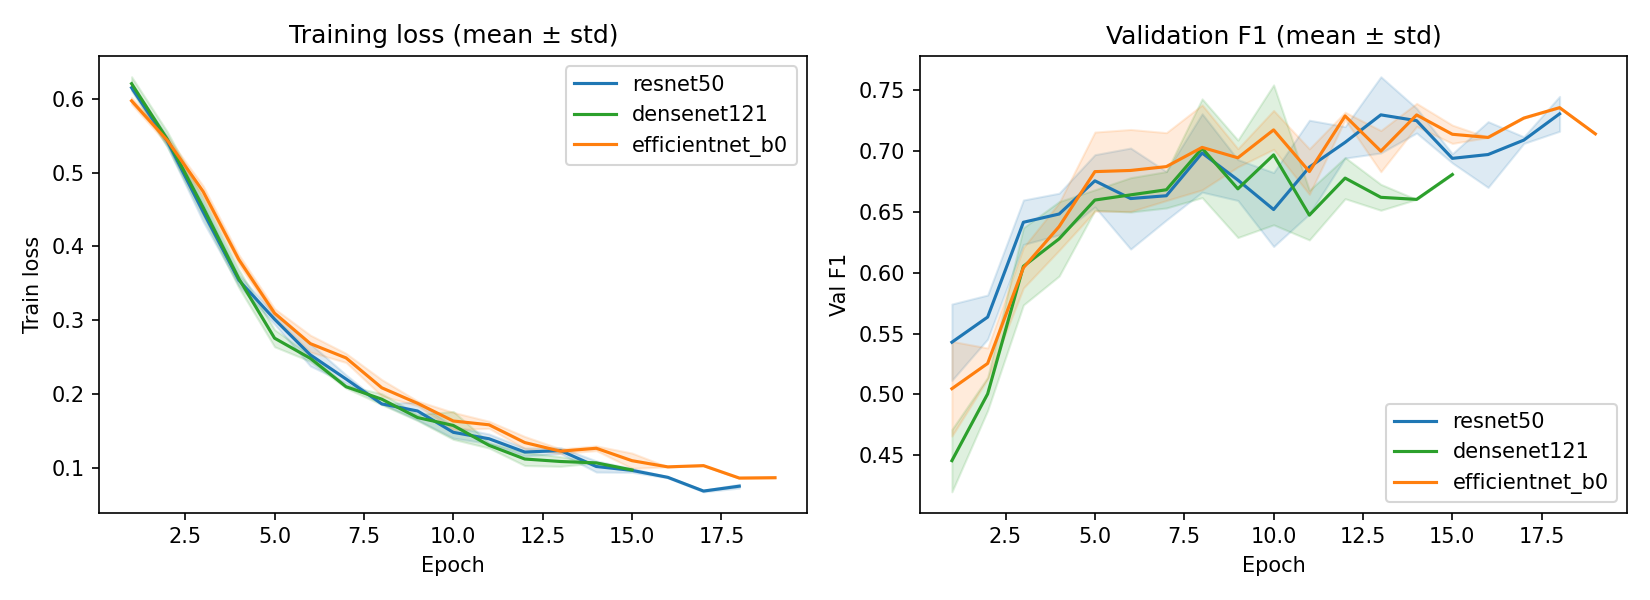
\includegraphics[width=0.92\textwidth]{learning_curves_combined.png}
\caption{Üç mimarinin tüm tohumlarda birleşik öğrenme eğrileri (doğrulama metrikleri). Modeller benzer bir doğruluk tavanına ulaşır.}
\label{fig:lc}
\end{figure*}

\begin{figure}[t]
\centering
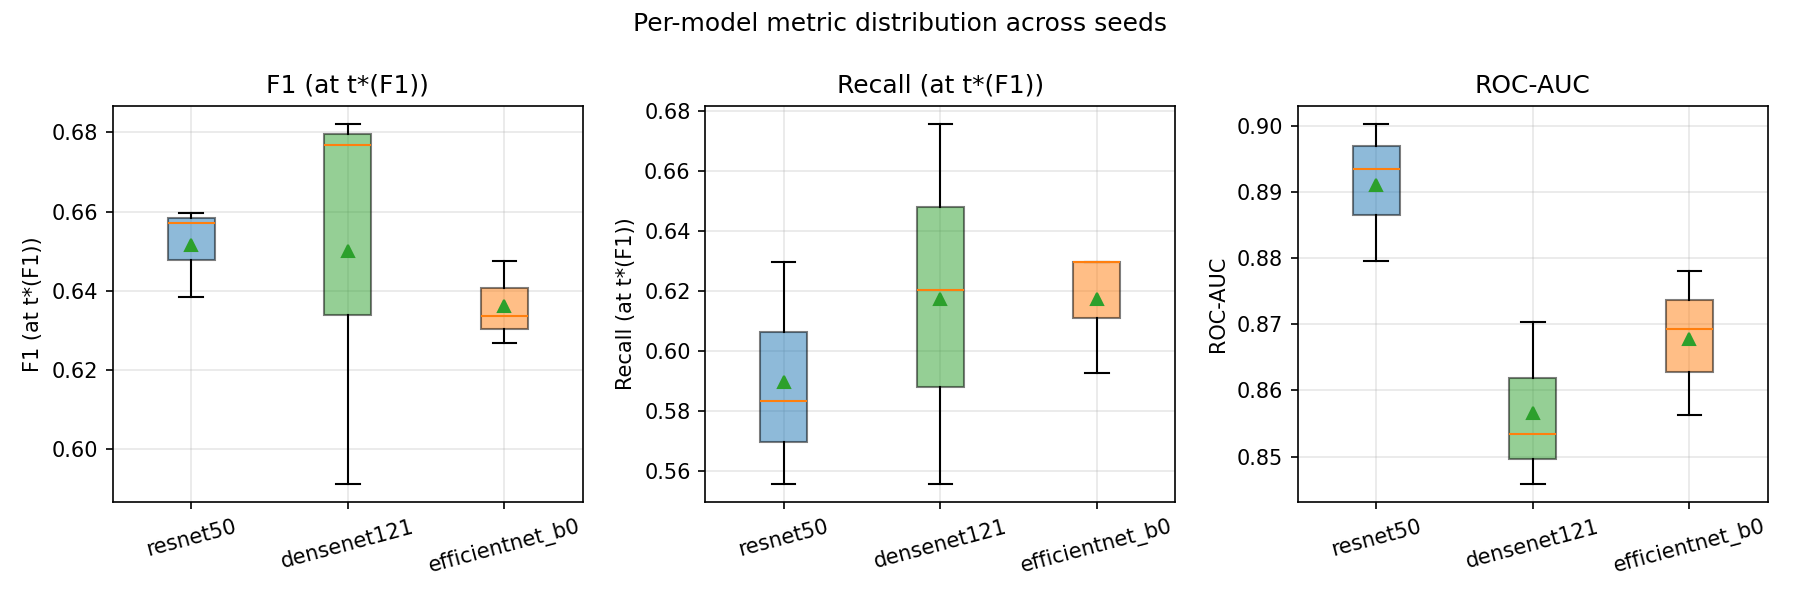
\includegraphics[width=\columnwidth]{metric_boxplot.png}
\caption{Metrik kutu grafiği (modeller $\times$ tohumlar). ResNet-50 hem en yüksek medyan F1/AUC'ye hem de en dar dağılıma sahiptir.}
\label{fig:box}
\end{figure}

\subsection{İstatistiksel Anlamlılık}
Modeller arası farkların gürültü düzeyinde olup olmadığını üç testle sınadık. \textbf{Eşli $t$-testi} (her tohum eşlenik gözlem, F1 @ $t=0.5$): ResNet-50'nin EfficientNet-B0'a F1 üstünlüğü \emph{anlamlıdır} ($t = 5.48$, $p = 0.032$); buna karşın ResNet-50 vs DenseNet-121 ($p = 0.32$) ve DenseNet-121 vs EfficientNet-B0 ($p = 0.35$) farkları anlamlı değildir. \textbf{DeLong testi} (ROC-AUC) ResNet-50'nin DenseNet-121'e AUC üstünlüğünü iki tohumda anlamlı bulmuştur ($p = 0.016$ ve $p = 0.015$). \textbf{McNemar testi} çoğu çiftte anlamlı fark vermemiştir. Sonuç: ResNet-50 azınlık sınıfı başarımında en güçlü ve en tutarlı modeldir; EfficientNet-B0 ile arasındaki fark istatistiksel olarak anlamlıdır. ROC eğrileri (Şekil~\ref{fig:roc}) bu sıralamayı destekler.

\begin{figure}[t]
\centering
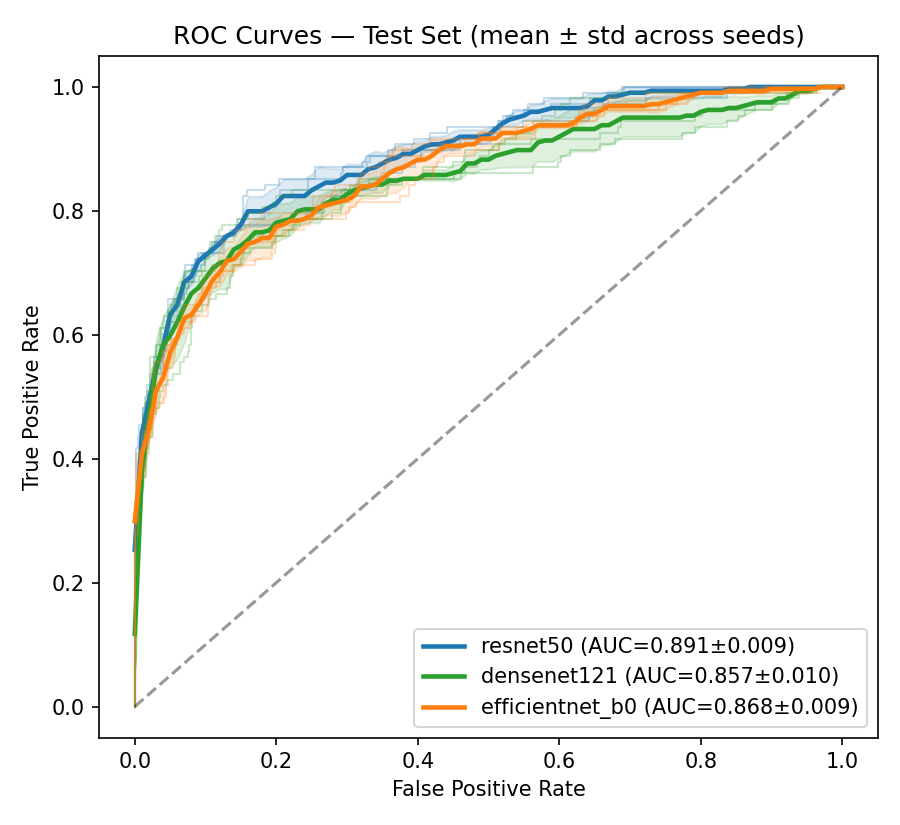
\includegraphics[width=\columnwidth]{roc_comparison_all_seeds.png}
\caption{ROC eğrisi karşılaştırması (tüm tohumlar). ResNet-50 en yüksek ortalama AUC'yi verir.}
\label{fig:roc}
\end{figure}

\subsection{Çalışma Noktası (Karar Eşiği) Analizi}
Sınıf dengesizliği nedeniyle karar eşiği seçimi precision--recall dengesini doğrudan belirler (Tablo~\ref{tab:thr}). Varsayılan $t = 0.5$ precision'ı yükseltirken recall'u sınırlar. \textbf{Youden} noktası ($t \approx 0.30$) kırık geri-çağırma oranını $0.667 \to 0.731$'e yükseltir; bu, kaçırılan kırığın maliyetli olduğu klinik senaryoda tercih edilebilir bir ödünleşimdir.

\begin{table}[t]
\caption{Çalışma Noktası Karşılaştırması --- ResNet-50 (3 Tohum Ort.)}
\label{tab:thr}
\centering
\begin{tabular}{lccccc}
\toprule
\textbf{Çalışma noktası} & \textbf{Eşik} & \textbf{Acc.} & \textbf{Prec.} & \textbf{Recall} & \textbf{F1} \\
\midrule
Varsayılan  & 0.50 & 0.888 & 0.688 & 0.667 & 0.677 \\
F1-optimal  & 0.69 & 0.889 & 0.732 & 0.590 & 0.652 \\
Youden      & 0.30 & 0.874 & 0.625 & $\mathbf{0.731}$ & 0.673 \\
\bottomrule
\end{tabular}
\end{table}

\subsection{Verimlilik}
Mimariler doğrulukta yakınken asıl fark verimlilikte ortaya çıkar (Tablo~\ref{tab:eff}). EfficientNet-B0, ResNet-50'nin yaklaşık $1/6$'sı parametresiyle (4.01M vs 23.51M) rekabetçi accuracy ve AUC sağlar. Bu, sınırlı kaynak veya gömülü/mobil dağıtım hedefi olan senaryolarda EfficientNet-B0'ın güçlü bir aday olduğunu gösterir; en yüksek azınlık-sınıfı başarımı öncelikliyse ResNet-50 tercih edilmelidir.

\begin{table}[t]
\caption{Verimlilik ve Model Karmaşıklığı (3 Çalışma Ort.)}
\label{tab:eff}
\centering
\begin{tabular}{lcccc}
\toprule
\textbf{Mimari} & \textbf{Param (M)} & \textbf{Epoch (s)} & \textbf{F1} & \textbf{ROC-AUC} \\
\midrule
ResNet-50      & 23.51 & 37.6 & $\mathbf{0.677}$ & $\mathbf{0.891}$ \\
DenseNet-121   & 6.96  & 40.0 & 0.651 & 0.857 \\
EfficientNet-B0 & $\mathbf{4.01}$ & 35.9 & 0.626 & 0.868 \\
\bottomrule
\end{tabular}
\end{table}

\begin{figure*}[t]
\centering
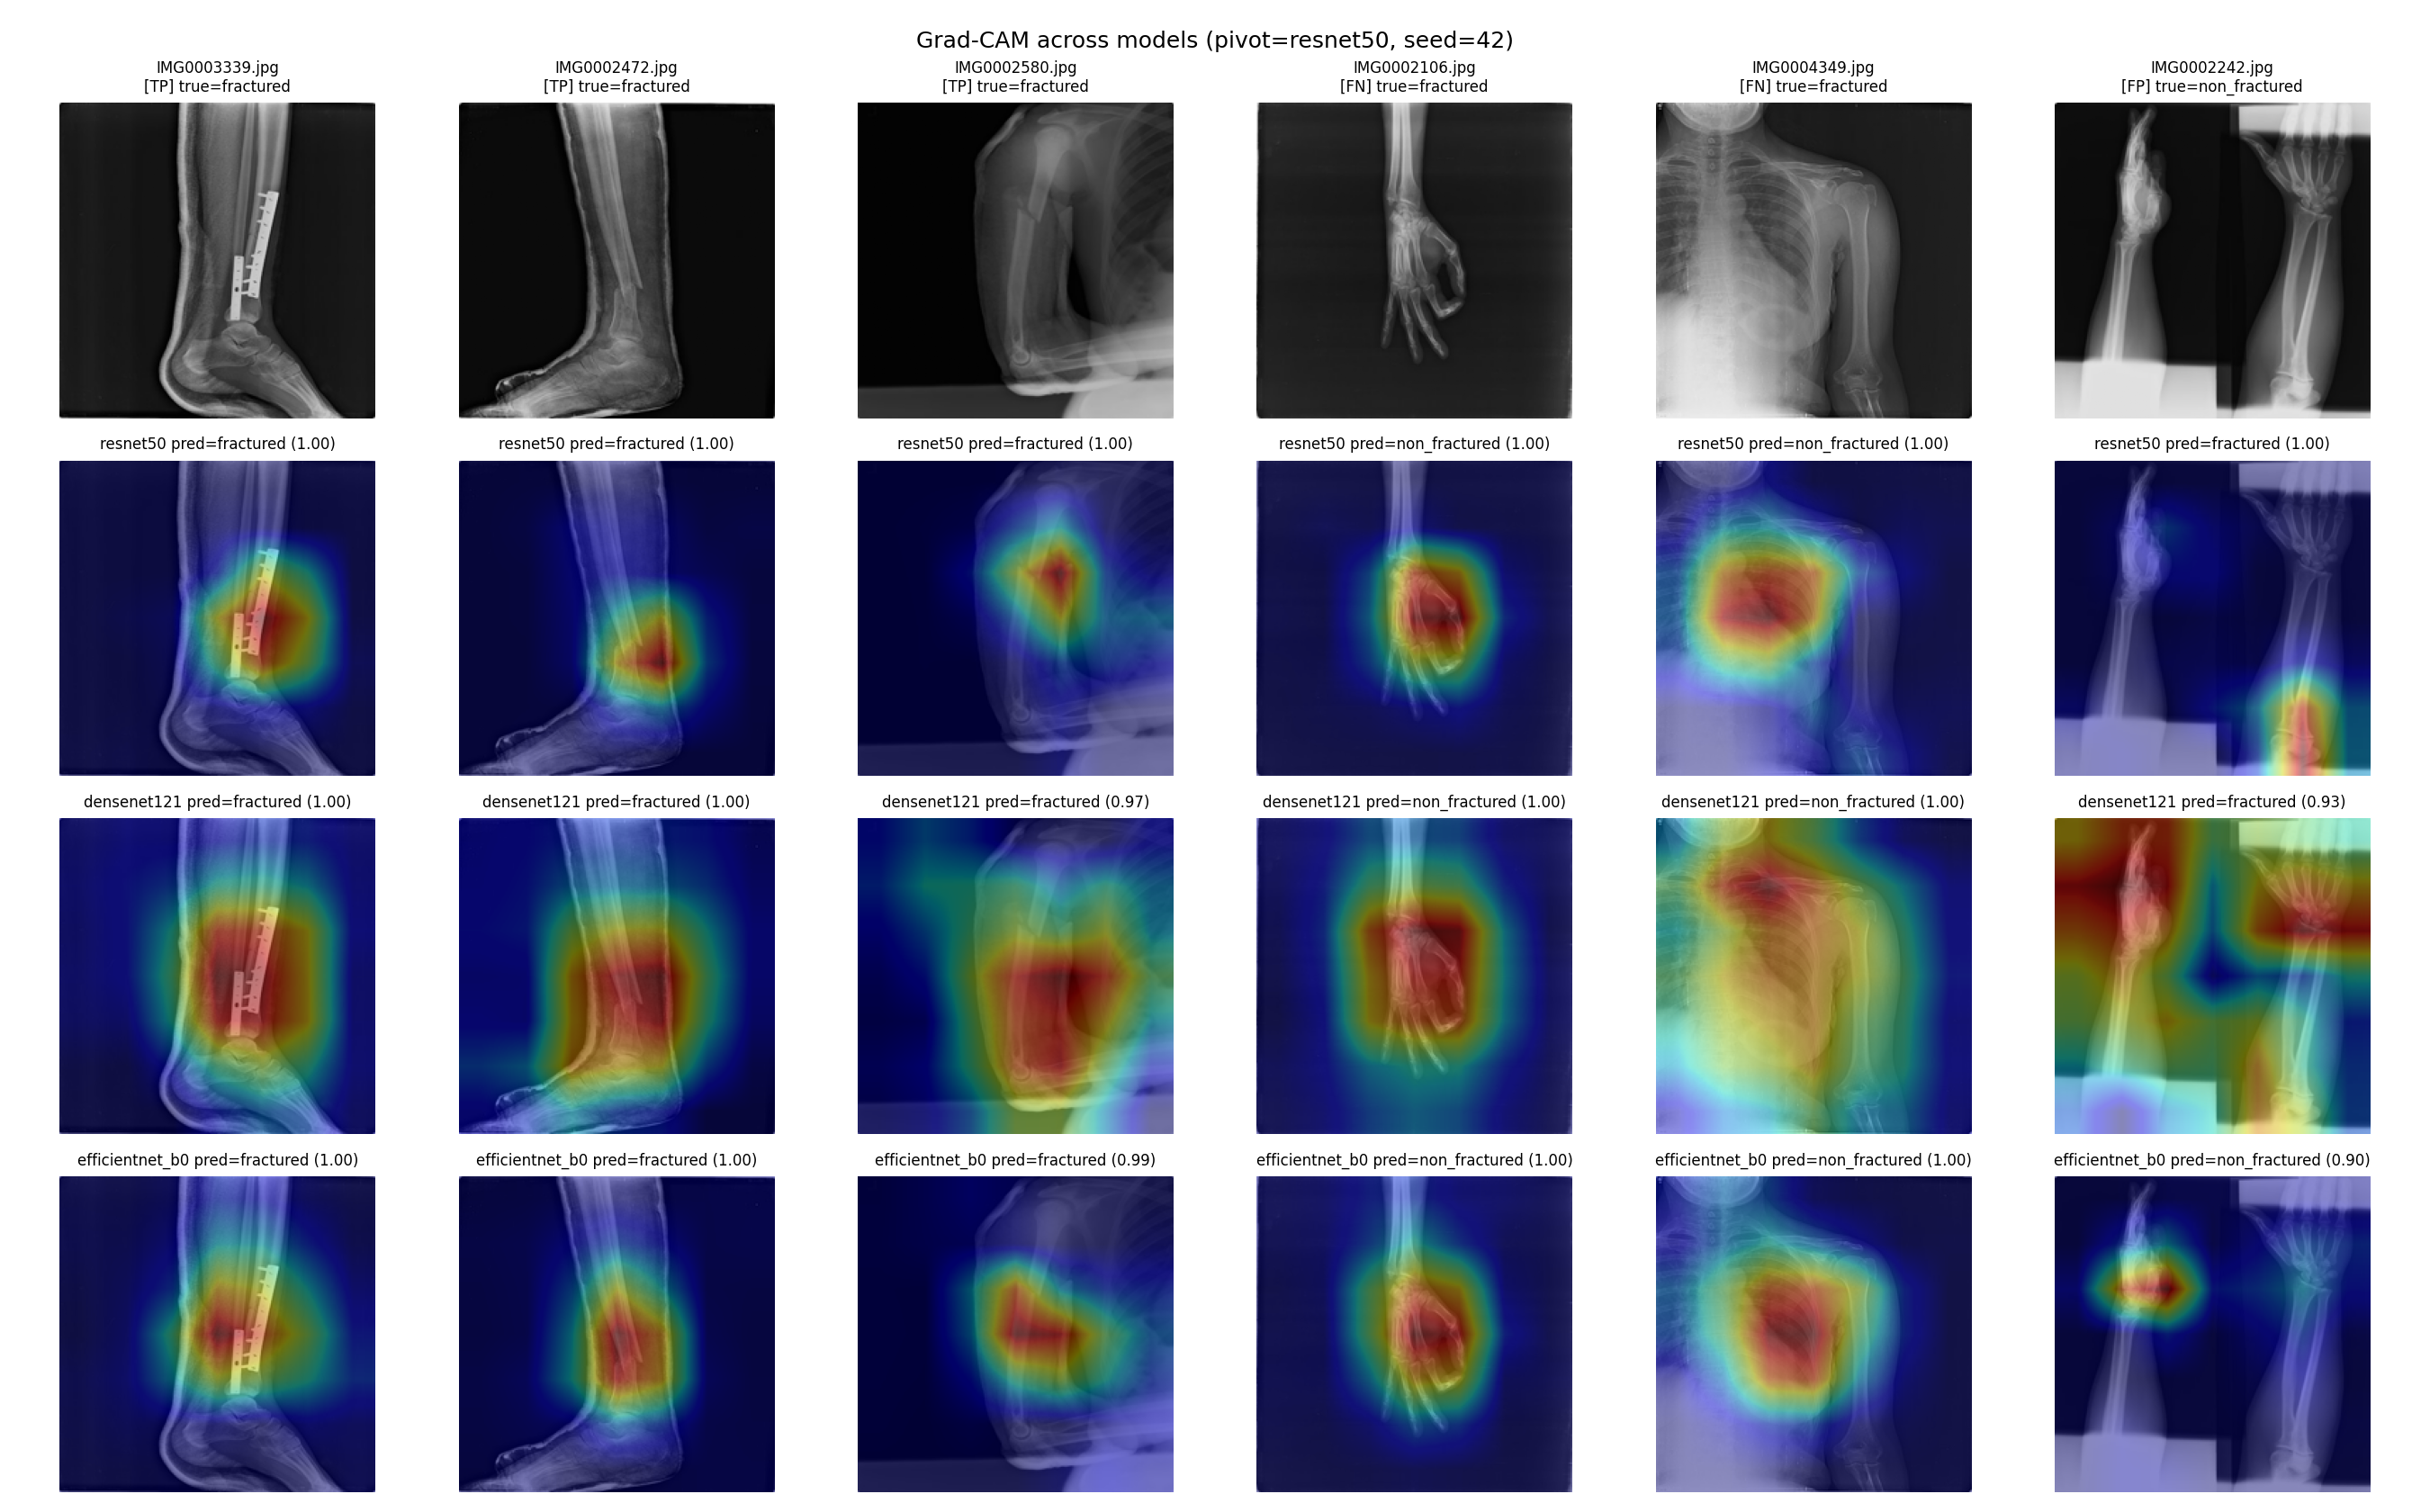
\includegraphics[width=0.92\textwidth]{gradcam_all_models_seed42.png}
\caption{Grad-CAM ısı haritaları (tohum 42). Doğru kararlarda etkinleşme kırık bölgesinde toplanır; hatalı örneklerde dağılır.}
\label{fig:gradcam}
\end{figure*}

\subsection{Hata Analizi (Karışıklık Matrisleri)}
Tablo~\ref{tab:cm}, tohum 42 için her mimarinin test karışıklık matrisini özetler. Üç modelde de hataların büyük kısmı kırığı kaçırma (yanlış negatif) biçimindedir; bu, dengesiz veride beklenen davranıştır ve azınlık sınıfının recall'unun neden darboğaz olduğunu açıklar. ResNet-50 en düşük FN (37) ile en yüksek kırık geri-çağırmasını sağlamıştır. Karışıklık matrislerinin görsel biçimi Şekil~\ref{fig:cm}'de verilmiştir.

\begin{table}[t]
\caption{Karışıklık Matrisleri --- Test Seti (Tohum 42)}
\label{tab:cm}
\centering
\begin{tabular}{lccccccc}
\toprule
\textbf{Mimari} & \textbf{TN} & \textbf{FP} & \textbf{FN} & \textbf{TP} & \textbf{F1} & \textbf{AUC} \\
\midrule
ResNet-50      & 475 & 30 & $\mathbf{37}$ & $\mathbf{71}$ & $\mathbf{0.679}$ & $\mathbf{0.880}$ \\
DenseNet-121   & 456 & 49 & 38 & 70 & 0.617 & 0.846 \\
EfficientNet-B0 & 468 & 37 & 41 & 67 & 0.632 & 0.869 \\
\bottomrule
\end{tabular}
\end{table}

\begin{figure}[t]
\centering
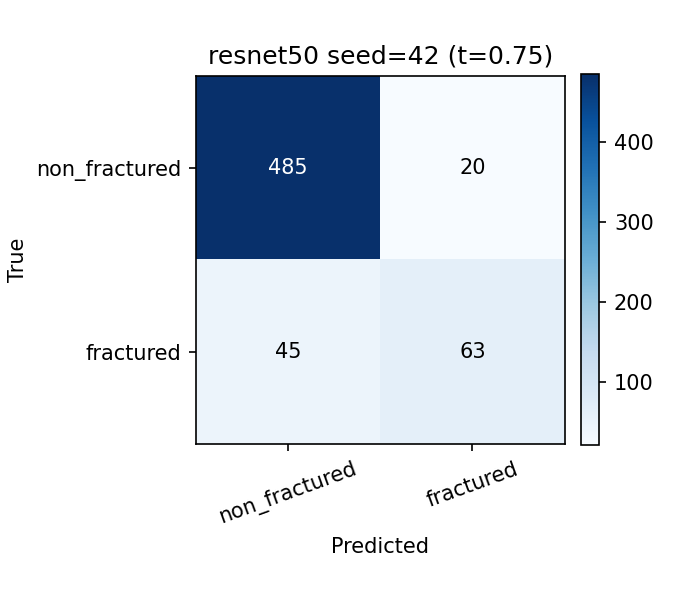
\includegraphics[width=0.32\columnwidth]{confusion_resnet50_seed42.png}\hfill
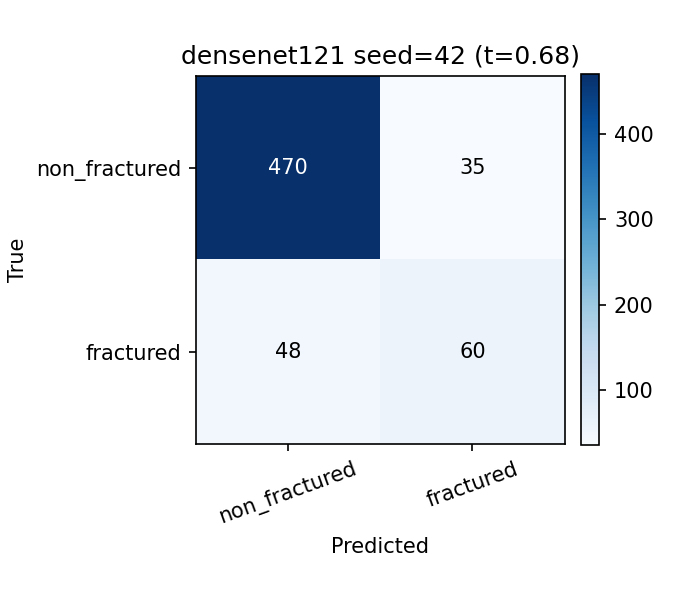
\includegraphics[width=0.32\columnwidth]{confusion_densenet121_seed42.png}\hfill
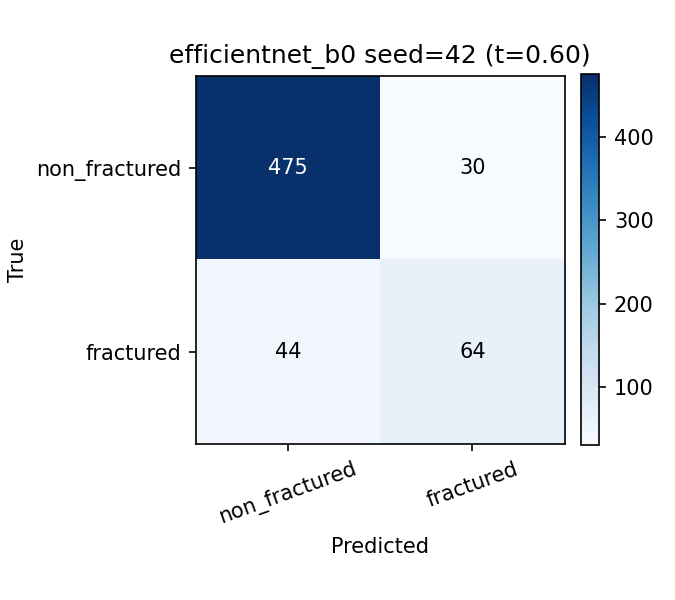
\includegraphics[width=0.32\columnwidth]{confusion_efficientnet_b0_seed42.png}
\caption{Karışıklık matrisleri (tohum 42): soldan sağa ResNet-50, DenseNet-121, EfficientNet-B0. Hataların çoğu yanlış negatif (kaçırılan kırık) yönündedir.}
\label{fig:cm}
\end{figure}

\subsection{Açıklanabilirlik (Grad-CAM)}
En iyi modelin (ResNet-50) kararlarını yorumlamak için son evrişim bloğu (\texttt{layer4}) üzerinden Grad-CAM ısı haritaları üretilmiştir (Şekil~\ref{fig:gradcam}). Doğru sınıflandırılan kırık örneklerinde ısı haritası tutarlı biçimde kırık/kortikal süreksizlik bölgesinde yoğunlaşmakta; modelin klinik olarak anlamlı bölgelere odaklandığını doğrulamaktadır. Hatalı örneklerde ise ısı haritası dağınıktır ya da kırık dışı yapılara kaymaktadır. Modelin sistematik kör noktaları ince/çizgisel kırıklar ve atipik görüntülerdir.

\section{Tartışma}
\textbf{Mimariler doğrulukta yakın, azınlık başarımında ayrışır.} ImageNet ön-eğitimli üç mimari, orta ölçekli ve dengesiz bu veride benzer bir doğruluk tavanına ulaşır. Asıl ayrım, dengesizlik altında azınlık sınıfı başarımında (F1/AUC) ortaya çıkar; burada ResNet-50 hem en yüksek hem en kararlı modeldir ve EfficientNet-B0'a üstünlüğü istatistiksel olarak anlamlıdır.

\textbf{Doğruluk $\neq$ verimlilik.} En yüksek azınlık başarımı (ResNet-50) ile en yüksek parametre verimliliği (EfficientNet-B0) farklı modellerde toplanmıştır. Dağıtım hedefi doğruluk öncelikliyse ResNet-50, kaynak/hız öncelikliyse EfficientNet-B0 tercih edilmelidir.

\textbf{Çalışma noktası tasarımı kritiktir.} Tek bir $0.5$ eşiğiyle raporlama dengesiz veride yanıltıcıdır; eşik seçimi aynı modelden çok farklı precision--recall dengeleri çıkarır. Klinik olarak kaçırılan kırığın maliyeti yüksek olduğundan, recall'u yükselten Youden noktası savunulabilir bir tercihtir.

\textbf{Açıklanabilirlik güveni artırır.} Grad-CAM, en iyi modelin doğru kararlarında kırık bölgesine odaklandığını göstererek modelin ``doğru nedenle doğru'' karar verdiğine dair kanıt sunar.

\textbf{Sınırlılıklar.} (i) Tek veri kümesi ve tek dahili bölme protokolü --- çapraz-veri genellemesi sınanmamıştır. (ii) Problem kırık var/yok ile sınırlıdır. (iii) K-katlamalı çapraz doğrulama yerine sabit bölme + çoklu tohum kullanılmıştır. (iv) Sınıf dengesizliği uçlarda (ince kırıklar) hatayı artırmaktadır.

\section{Sonuç}
FracAtlas üzerinde üç CNN mimarisini ortak transfer öğrenme çatısında, çok-tohumlu ve istatistiksel olarak sınanmış biçimde karşılaştıran kontrollü bir çalışma sunduk. Mimariler genel doğrulukta yakındır; ancak dengesiz veride asıl belirleyici olan azınlık (kırık) sınıfı başarımında \textbf{ResNet-50 en yüksek F1 (0.677) ve ROC-AUC (0.891) değerini vermiş} ve EfficientNet-B0'a F1 üstünlüğü istatistiksel olarak anlamlı bulunmuştur ($p = 0.032$). EfficientNet-B0 ise $\approx 1/6$ parametreyle verimlilik ekseninde öne çıkmıştır. Karar eşiği analizi Youden noktasıyla kırık geri-çağırmasının $0.73$'e yükseltilebildiğini; Grad-CAM analizi ise en iyi modelin kırık bölgesine odaklandığını göstermiştir. Gelecek çalışmalar: çapraz-veri değerlendirmesi (örn. MURA), kırık tipi/konumu için çok-sınıflı veya tespit tabanlı genişletme, odak (focal) kayıp gibi dengesizliğe özgü kayıplar ve daha güçlü mimarilerin (ConvNeXt, Vision Transformer) eklenmesi.

\begin{thebibliography}{00}
\bibitem{fracatlas} I. Abedeen, M. A. Rahman, F. Z. Prottyasha, T. Ahmed, T. M. Chowdhury, and S. Shatabda, ``FracAtlas: A dataset for fracture classification, localization and segmentation of musculoskeletal radiographs,'' \emph{Scientific Data}, vol. 10, art. 521, 2023.
\bibitem{resnet} K. He, X. Zhang, S. Ren, and J. Sun, ``Deep residual learning for image recognition,'' in \emph{Proc. IEEE CVPR}, 2016, pp. 770--778.
\bibitem{densenet} G. Huang, Z. Liu, L. van der Maaten, and K. Q. Weinberger, ``Densely connected convolutional networks,'' in \emph{Proc. IEEE CVPR}, 2017, pp. 4700--4708.
\bibitem{efficientnet} M. Tan and Q. Le, ``EfficientNet: Rethinking model scaling for convolutional neural networks,'' in \emph{Proc. ICML}, 2019, pp. 6105--6114.
\bibitem{imagenet} J. Deng, W. Dong, R. Socher, L.-J. Li, K. Li, and L. Fei-Fei, ``ImageNet: A large-scale hierarchical image database,'' in \emph{Proc. IEEE CVPR}, 2009, pp. 248--255.
\bibitem{gradcam} R. R. Selvaraju, M. Cogswell, A. Das, R. Vedantam, D. Parikh, and D. Batra, ``Grad-CAM: Visual explanations from deep networks via gradient-based localization,'' in \emph{Proc. IEEE ICCV}, 2017, pp. 618--626.
\bibitem{mura} P. Rajpurkar et al., ``MURA: Large dataset for abnormality detection in musculoskeletal radiographs,'' in \emph{Proc. MIDL}, 2018.
\bibitem{lindsey} R. Lindsey et al., ``Deep neural network improves fracture detection by clinicians,'' \emph{Proc. Natl. Acad. Sci. USA}, vol. 115, no. 45, pp. 11591--11596, 2018.
\bibitem{kim} D. H. Kim and T. MacKinnon, ``Artificial intelligence in fracture detection: transfer learning from deep convolutional neural networks,'' \emph{Clinical Radiology}, vol. 73, no. 5, pp. 439--445, 2018.
\bibitem{adamw} I. Loshchilov and F. Hutter, ``Decoupled weight decay regularization,'' in \emph{Proc. ICLR}, 2019.
\bibitem{tajbakhsh} N. Tajbakhsh et al., ``Convolutional neural networks for medical image analysis: Full training or fine tuning?,'' \emph{IEEE Trans. Med. Imaging}, vol. 35, no. 5, pp. 1299--1312, 2016.
\bibitem{delong} E. R. DeLong, D. M. DeLong, and D. L. Clarke-Pearson, ``Comparing the areas under two or more correlated ROC curves: a nonparametric approach,'' \emph{Biometrics}, vol. 44, no. 3, pp. 837--845, 1988.
\bibitem{mcnemar} Q. McNemar, ``Note on the sampling error of the difference between correlated proportions or percentages,'' \emph{Psychometrika}, vol. 12, no. 2, pp. 153--157, 1947.
\bibitem{buda} M. Buda, A. Maki, and M. A. Mazurowski, ``A systematic study of the class imbalance problem in convolutional neural networks,'' \emph{Neural Networks}, vol. 106, pp. 249--259, 2018.
\bibitem{paplham} J. Paplham and V. Franc, ``A call to reflect on evaluation practices for age estimation,'' \emph{arXiv:2307.04570}, 2023.
\bibitem{augment} C. Shorten and T. M. Khoshgoftaar, ``A survey on image data augmentation for deep learning,'' \emph{Journal of Big Data}, vol. 6, art. 60, 2019.
\bibitem{litjens} G. Litjens et al., ``A survey on deep learning in medical image analysis,'' \emph{Medical Image Analysis}, vol. 42, pp. 60--88, 2017.
\end{thebibliography}

\end{document}
